\chapter{Des matières premières au recyclage}\label{ch:g5:raw-materials-and-recycling}

Une canette vide tombe dans un bac de \omterm{def:g5:raw-materials-and-recycling:recycling}{recyclage}. Un camion l'emporte
vers un centre de tri, une machine l'écrase en un bloc avec des milliers
d'autres, un four fait fondre les blocs, et quelques semaines plus tard
le métal est de retour dans les rayons d'un magasin, sous la forme d'une
nouvelle canette. D'où venait ce métal au départ, et pourquoi vaut-il la
peine de faire fondre de vieilles canettes plutôt que de fabriquer du
métal neuf~?

\begin{recall}
Un objet est une chose que l'on peut voir et toucher~; son matériau est
ce dont il est fait --- bois, métal, verre, plastique, papier, tissu,
pierre (\cref{ch:g1:materials-around-us}). Au cours d'une \omterm{def:g5:irreversible-changes:chemical-change}{transformation
chimique}, de nouvelles substances apparaissent et il n'y a pas de chemin
de retour simple (\cref{ch:g5:irreversible-changes}).
\end{recall}

\section{Matériaux naturels et matériaux fabriqués}

\begin{definition}[Matériaux naturels et matériaux fabriqués]\label{def:g5:raw-materials-and-recycling:natural-material}
Un \emph{matériau naturel}\index{materiau naturel@matériau naturel} s'utilise à peu près
tel qu'on le trouve dans la nature, simplement découpé ou façonné~: le
bois, la pierre, le coton, la laine, le cuir. Un
\emph{matériau fabriqué}\index{materiau fabrique@matériau fabriqué} est fabriqué par
l'être humain à partir de substances trouvées dans la nature, en les
transformant, souvent à l'aide de la chaleur et de \omterm{def:g5:irreversible-changes:chemical-change}{transformations
chimiques}~: le verre, l'acier, l'aluminium, le plastique, le papier, le
béton.
\end{definition}

\begin{example}[Deux tables]\label{ex:g5:raw-materials-and-recycling:tables}
Une table en planches de chêne est faite d'un \omterm{def:g5:raw-materials-and-recycling:natural-material}{matériau naturel}~: le bois
a seulement été scié, raboté et collé. Une table au plateau de verre et
aux pieds d'acier est faite de matériaux fabriqués~: on ne trouve tel
quel dans la nature ni le verre ni l'acier.
\end{example}

\section{Les matières premières}

\begin{definition}[Matière première et minerai]\label{def:g5:raw-materials-and-recycling:raw-material}
Une \emph{matière première}\index{matiere premiere@matière première} est une substance
prélevée dans la nature pour fabriquer des matériaux et des objets~: les
arbres, le sable, les roches, le pétrole brut, le coton, la laine. Une
roche dont on extrait un métal s'appelle un \emph{minerai}\index{minerai}.
\end{definition}

\begin{example}[D'où viennent les matériaux]\label{ex:g5:raw-materials-and-recycling:from}
\begin{itemize}
  \item le bois et le papier viennent des arbres~;
  \item le verre vient du sable, chauffé très fort avec de la soude et
        du calcaire~;
  \item le fer et l'acier viennent du \omterm{def:g5:raw-materials-and-recycling:raw-material}{minerai} de fer, une roche
        rougeâtre~;
  \item l'aluminium vient de la bauxite, un autre \omterm{def:g5:raw-materials-and-recycling:raw-material}{minerai}~;
  \item la plupart des plastiques viennent du pétrole brut, pompé dans le
        sous-sol~;
  \item le coton vient d'une plante, la laine des moutons.
\end{itemize}
\end{example}

\begin{omfigure}
\begin{minipage}[b]{0.48\linewidth}\centering
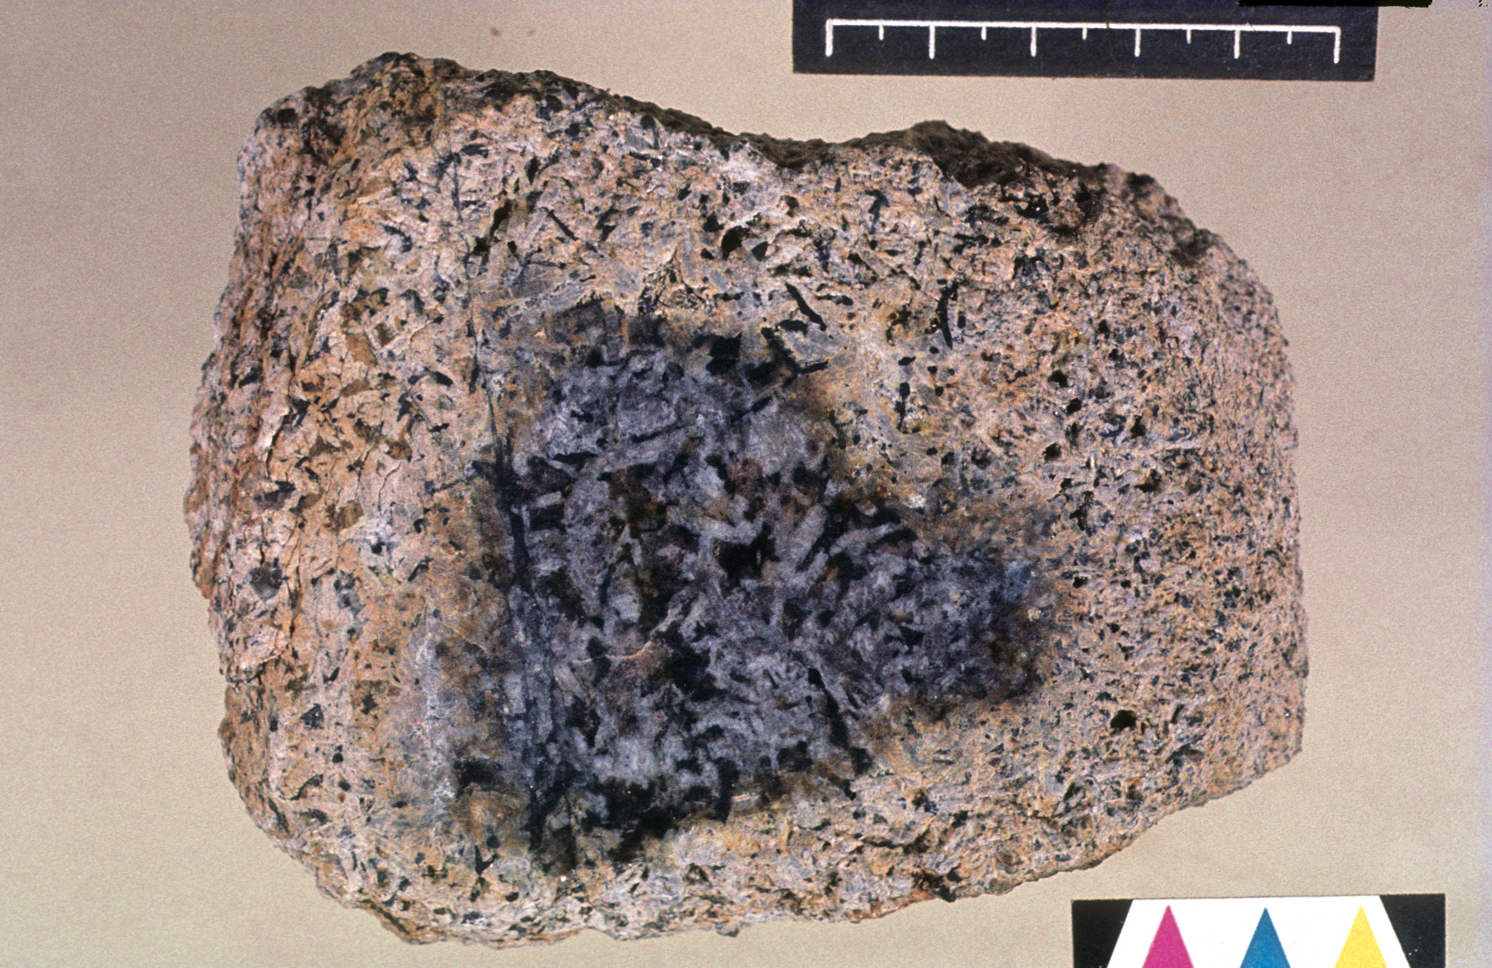
\includegraphics[width=\linewidth,height=4.6cm,keepaspectratio]{images/book1/bauxite.jpg}

{\small De la bauxite, le \omterm{def:g5:raw-materials-and-recycling:raw-material}{minerai} de l'aluminium, autour d'un cœur de
roche non altérée. Photo~: Werner Schellmann, CC BY-SA 2.5.}
\end{minipage}\hfill
\begin{minipage}[b]{0.48\linewidth}\centering
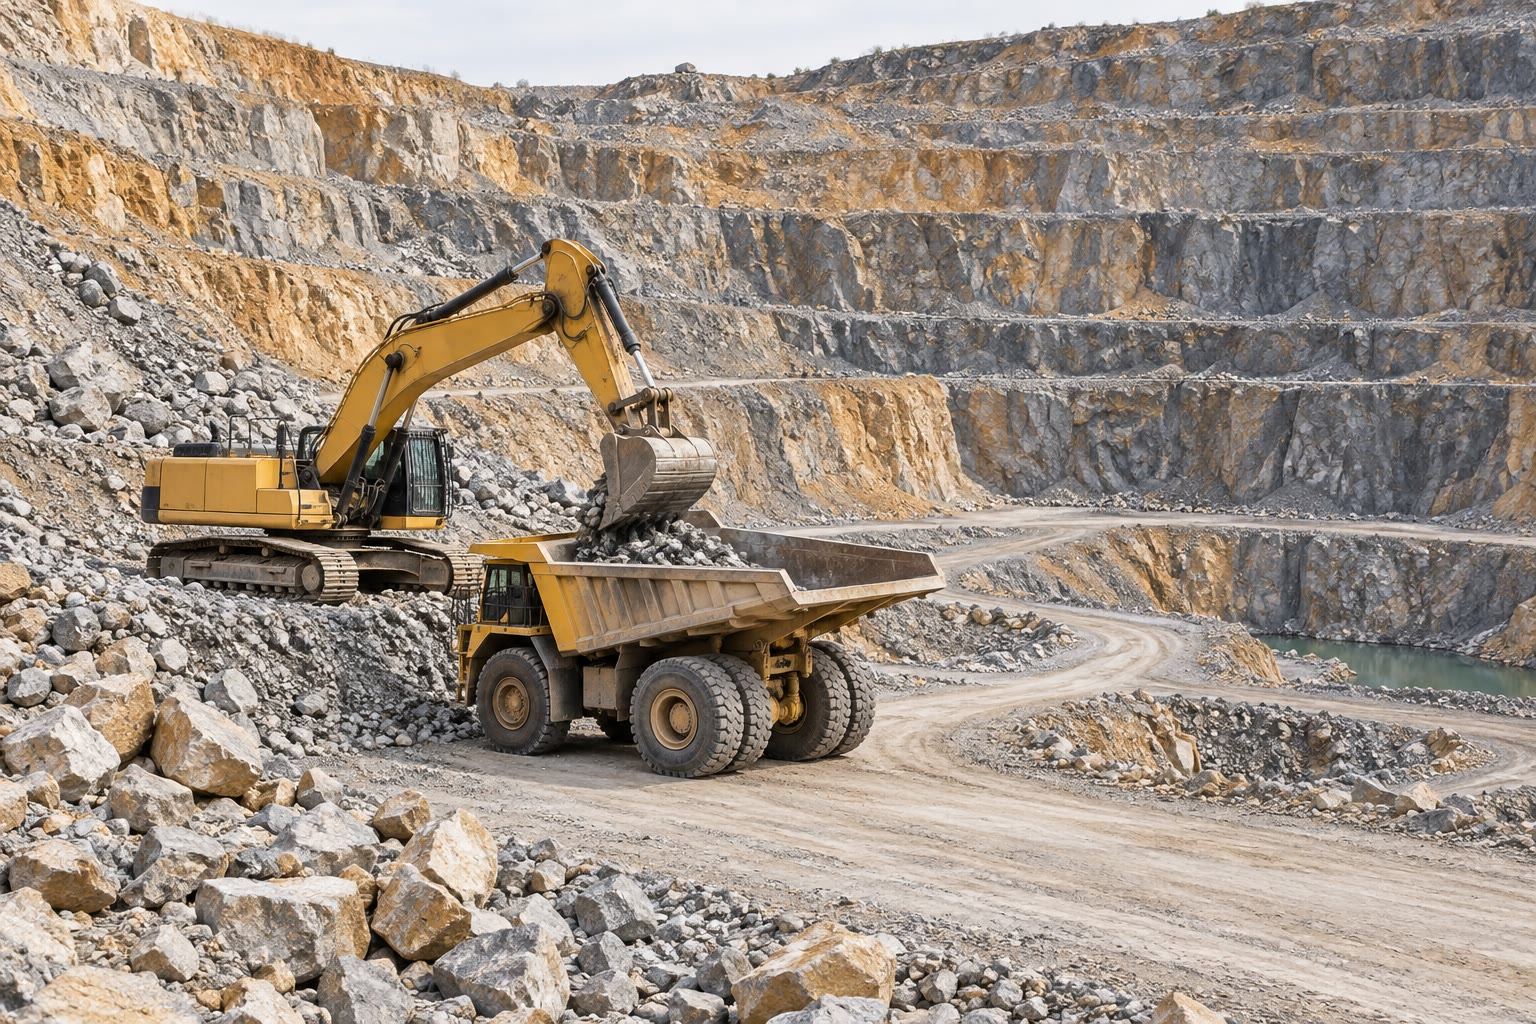
\includegraphics[width=\linewidth,height=4.6cm,keepaspectratio]{images/book1/ai/g5-quarry.jpg}

{\small Une carrière~: on y extrait la roche pour l'utiliser comme
\omterm{def:g5:raw-materials-and-recycling:raw-material}{matière première}.}
\end{minipage}
\end{omfigure}

\begin{omfigure}
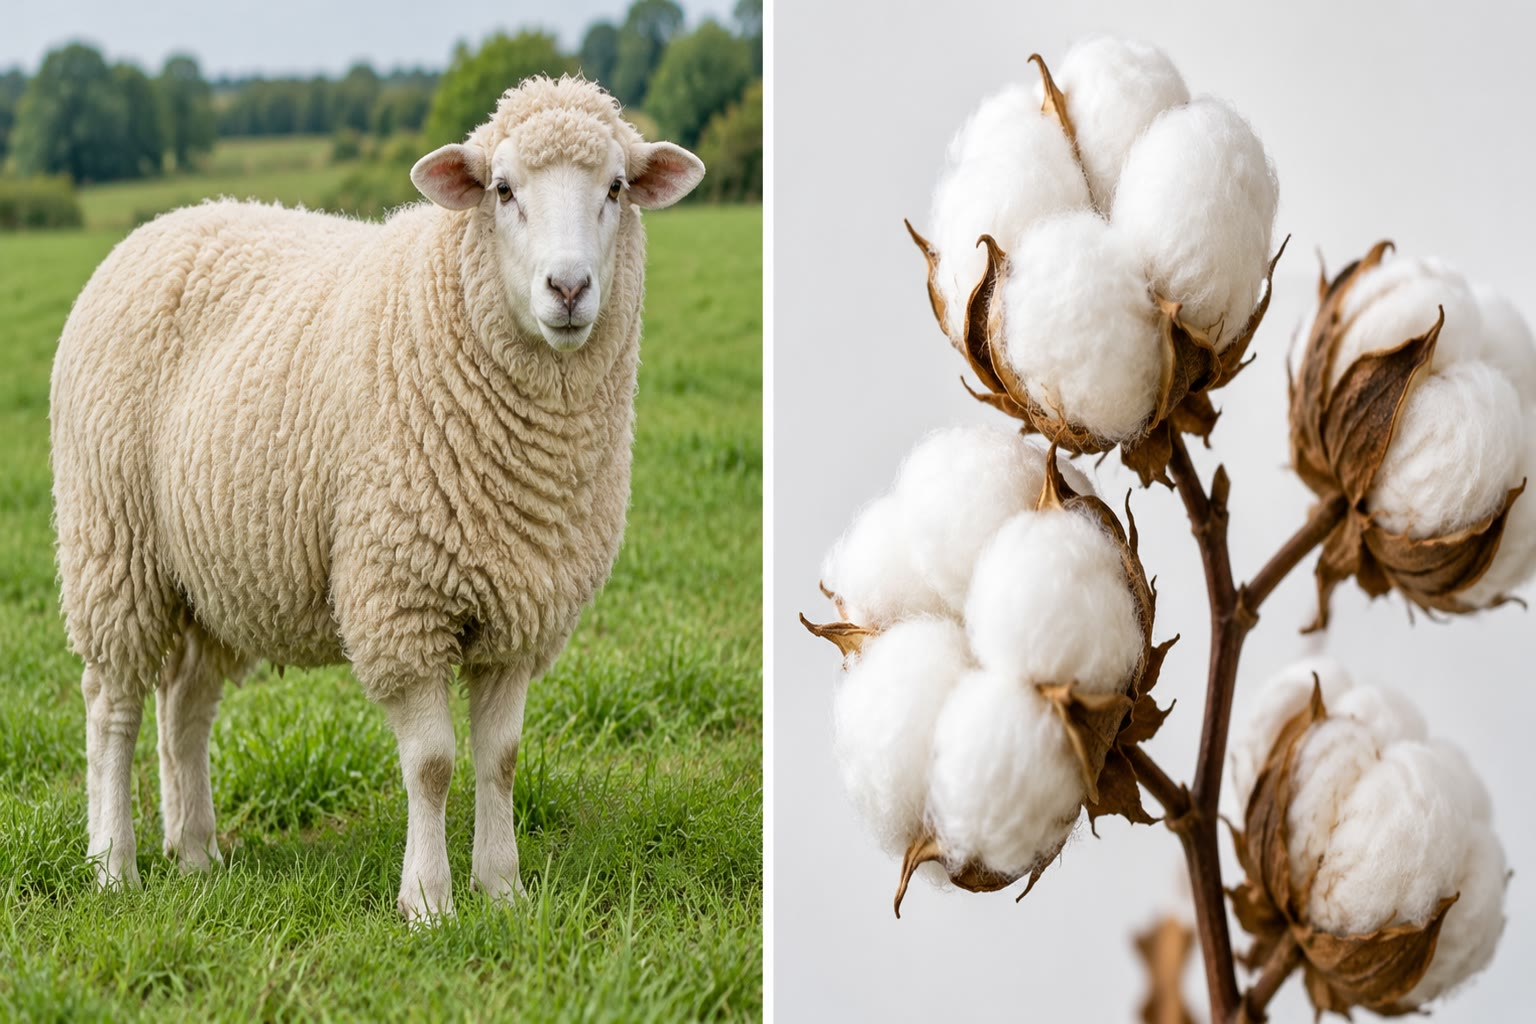
\includegraphics[width=0.6\linewidth]{images/book1/ai/g5-sheep-cotton.jpg}

{\small Des \omterm{def:g5:raw-materials-and-recycling:raw-material}{matières premières} naturelles venues d'êtres vivants~: la
laine des moutons, le coton du cotonnier.}
\end{omfigure}

\section{De la matière première à l'objet}

\begin{proposition}[Fabriquer un matériau transforme sa matière première]\label{prop:g5:raw-materials-and-recycling:change}
Transformer une \omterm{def:g5:raw-materials-and-recycling:raw-material}{matière première} en \omterm{def:g5:raw-materials-and-recycling:natural-material}{matériau fabriqué} demande de
l'énergie --- le plus souvent la chaleur d'un four --- et en général des
\omterm{def:g5:irreversible-changes:chemical-change}{transformations chimiques}~: le sable devient du verre, le \omterm{def:g5:raw-materials-and-recycling:raw-material}{minerai} devient
du métal, le pétrole devient du plastique. Ces transformations ne
peuvent pas être défaites simplement~: le verre ne redevient pas du
sable.
\end{proposition}

\begin{example}[La vie d'une bouteille en verre]\label{ex:g5:raw-materials-and-recycling:bottle}
On chauffe ensemble dans un four du sable, de la soude et du calcaire
broyé jusqu'à ce qu'ils fondent en verre. On souffle le verre chaud pour
lui donner la forme d'une bouteille. La bouteille est remplie, vendue et
vidée. Déposée dans un conteneur à verre, elle est broyée en petits
morceaux, fondue de nouveau et soufflée en une nouvelle bouteille~: le
verre sert encore et encore.
\end{example}

\begin{omfigure}
\begin{tikzpicture}[font=\small,
    box/.style={draw=omDef, fill=omDef!6, rounded corners=2pt, align=center,
      minimum height=0.95cm, text width=2.4cm}]
  \node[box] (r) at (0,2.6) {matière première\\ (sable, minerai, pétrole)};
  \node[box] (m) at (4.0,2.6) {fabrication\\ du matériau};
  \node[box] (o) at (8.0,2.6) {objet,\\ utilisé};
  \node[box] (w) at (8.0,0) {déchet};
  \node[box, draw=omProp, fill=omProp!8] (s) at (4.0,0) {tri et\\ recyclage};
  \draw[->, thick, omDef] (r) -- (m);
  \draw[->, thick, omDef] (m) -- (o);
  \draw[->, thick, omDef] (o) -- (w);
  \draw[->, thick, omProp] (w) -- (s);
  \draw[->, thick, omProp] (s) -- (m) node[midway, right, align=left, text=black]
    {réutilisé à la\\ place d'une\\ matière neuve};
  \draw[->, thick, black!45, dashed] (w.east) -- ++(1.4,0) node[right, align=left,
    text=black] {jeté~:\\ décharge};
\end{tikzpicture}

{\small La vie d'un matériau. La boucle orange est le \omterm{def:g5:raw-materials-and-recycling:recycling}{recyclage}~: le
matériau d'un vieil objet remplace une \omterm{def:g5:raw-materials-and-recycling:raw-material}{matière première} neuve.}
\end{omfigure}

\section{Trier et recycler}

\begin{definition}[Recyclage]\label{def:g5:raw-materials-and-recycling:recycling}
Le \emph{recyclage}\index{recyclage} consiste à collecter les objets
usagés et à traiter leur matériau pour en faire de nouveaux objets, au
lieu de le jeter.
\end{definition}

\begin{proposition}[Pourquoi recycler]\label{prop:g5:raw-materials-and-recycling:why}
% ledger: al:energy-primary, al:energy-recycled (8.3 / 186 = about 1/22)
Le \omterm{def:g5:raw-materials-and-recycling:recycling}{recyclage} économise des \omterm{def:g5:raw-materials-and-recycling:raw-material}{matières premières}, qu'il n'est plus
nécessaire d'extraire du sous-sol, et il économise souvent de
l'énergie. Fabriquer de l'aluminium à partir de vieilles canettes ne
demande qu'environ un vingtième de l'énergie nécessaire pour le
fabriquer à partir de bauxite. Il y a aussi moins de déchets dans les
décharges.
\end{proposition}

\begin{method}[Trier les déchets pour le recyclage]\label{met:g5:raw-materials-and-recycling:sort}
Le \omterm{def:g5:raw-materials-and-recycling:recycling}{recyclage} commence par le tri, là où l'on jette les déchets~:
\begin{enumerate}
  \item les bouteilles et les bocaux en verre dans un bac~;
  \item les canettes en métal, le papier et le carton, et les bouteilles
        en plastique dans les bacs que la commune prévoit pour eux (la
        couleur des bacs change d'un endroit à l'autre)~;
  \item ce qui ne se recycle pas avec le reste des déchets.
\end{enumerate}
Chaque matériau se recycle à sa façon~: un bac ne doit donc contenir que
les matériaux auxquels il est destiné.
\end{method}

\begin{omfigure}
\begin{tikzpicture}[font=\small]
  \foreach \k/\t/\bc in {0/verre/green!50!black, 1/{canettes en métal}/gray,
                        2/{papier et carton}/omDef, 3/{bouteilles en plastique}/orange!80!black} {
    \begin{scope}[xshift=\k*3.4cm]
      \fill[\bc!18, draw=\bc, line width=0.8pt] (-1,0) -- (1,0) -- (1.15,2.0)
        -- (-1.15,2.0) -- cycle;
      \fill[\bc!45, draw=\bc] (-1.25,2.0) rectangle (1.25,2.3);
      \node[anchor=north, align=center] at (0,-0.15) {\t};
    \end{scope}
  }
  % glass: a bottle
  \fill[green!40!black!60] (-0.2,0.3) rectangle (0.2,1.2);
  \fill[green!40!black!60] (-0.07,1.2) rectangle (0.07,1.6);
  % metal: a can
  \begin{scope}[xshift=3.4cm]
    \fill[black!25, draw=black!55] (-0.3,0.3) rectangle (0.3,1.3);
  \end{scope}
  % paper: a box and a sheet
  \begin{scope}[xshift=6.8cm]
    \fill[brown!25, draw=brown!60] (-0.6,0.3) rectangle (0.1,1.0);
    \fill[white, draw=black!40] (0.2,0.3) rectangle (0.65,1.3);
  \end{scope}
  % plastic: a bottle
  \begin{scope}[xshift=10.2cm]
    \fill[cyan!20, draw=cyan!50!black] (-0.25,0.3) rectangle (0.25,1.3);
    \fill[cyan!20, draw=cyan!50!black] (-0.1,1.3) rectangle (0.1,1.6);
  \end{scope}
\end{tikzpicture}

{\small Quatre bacs de tri, un par matériau. (La couleur des vrais bacs
change d'une commune à l'autre.)}
\end{omfigure}

\begin{omfigure}
\begin{minipage}[t]{0.48\linewidth}\centering
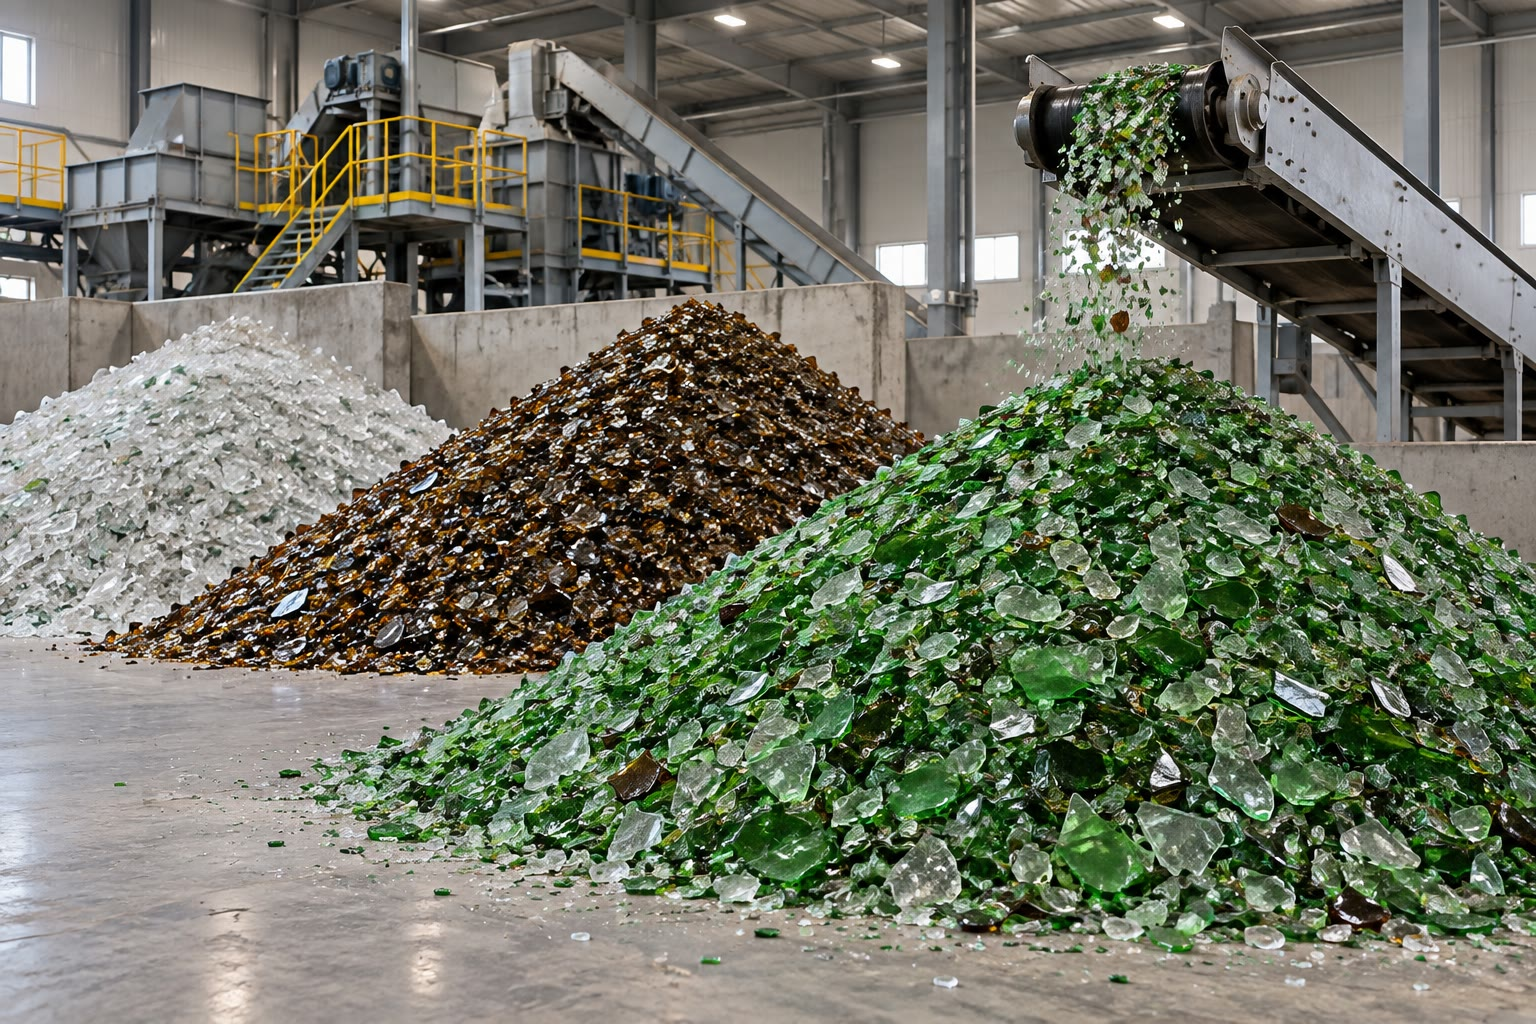
\includegraphics[width=\linewidth,height=4.6cm,keepaspectratio]{images/book1/ai/g5-glass-cullet.jpg}

{\small Du verre broyé dans une usine de \omterm{def:g5:raw-materials-and-recycling:recycling}{recyclage}, prêt à être fondu.}
\end{minipage}\hfill
\begin{minipage}[t]{0.48\linewidth}\centering
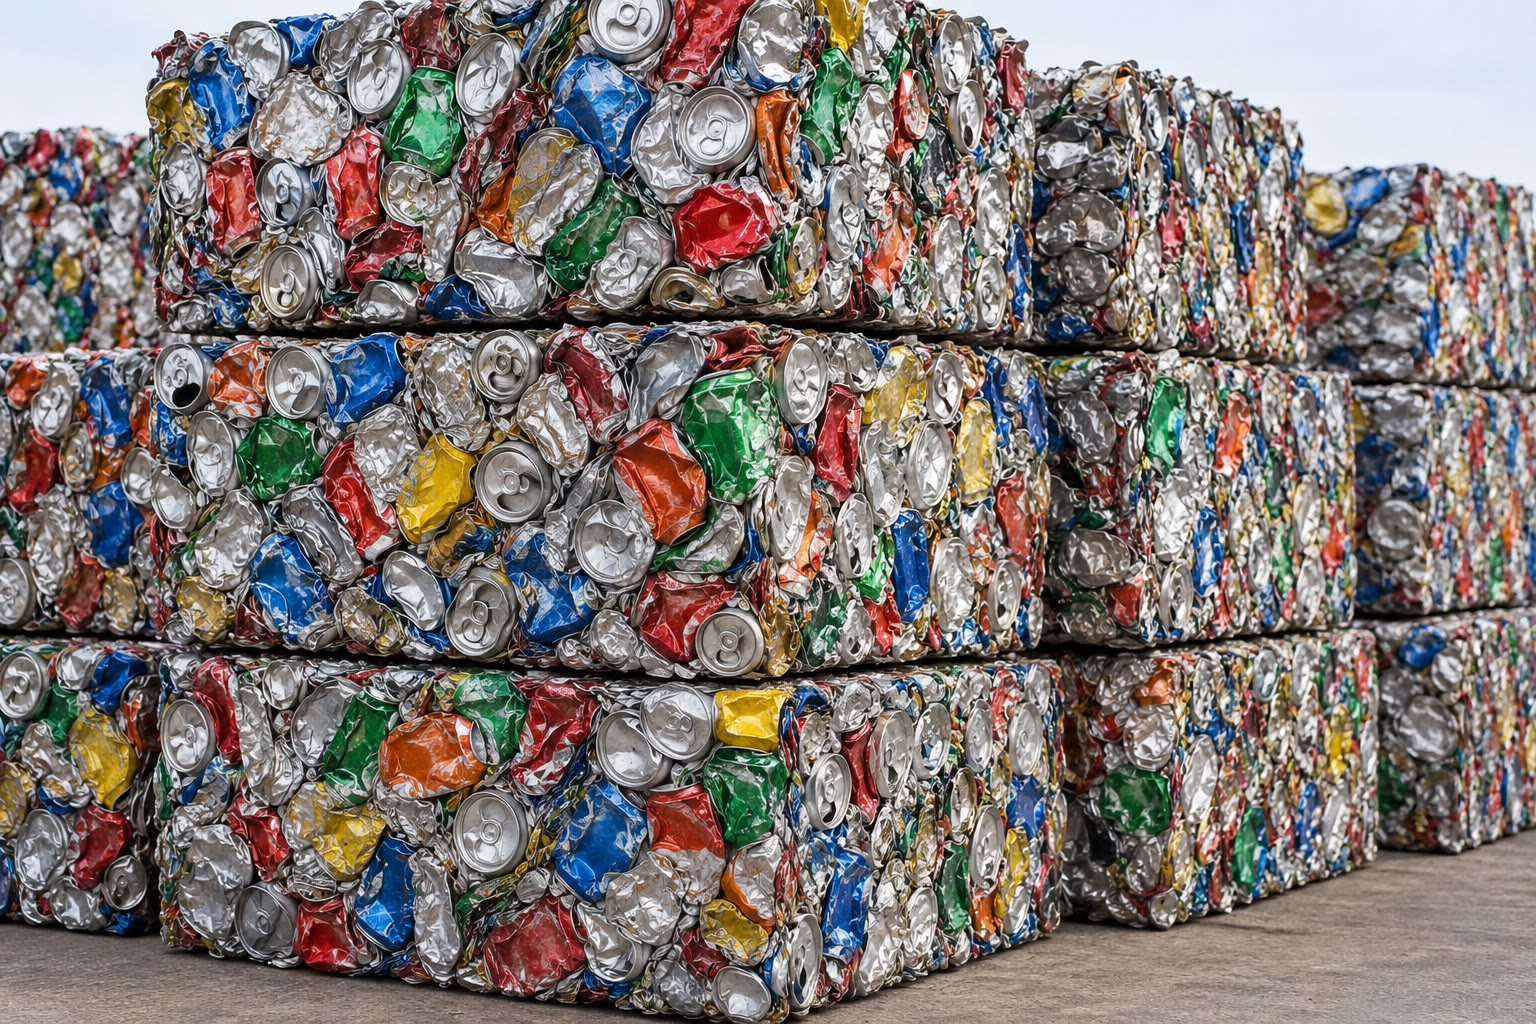
\includegraphics[width=\linewidth,height=4.6cm,keepaspectratio]{images/book1/ai/g5-can-bales.jpg}

{\small Des balles de canettes d'aluminium écrasées.}
\end{minipage}
\end{omfigure}

\section{Déchets et ressources}

\begin{definition}[Ressource]\label{def:g5:raw-materials-and-recycling:resource}
Une \emph{ressource}\index{ressource} est tout ce que l'on prélève dans la
nature pour l'utiliser~: l'eau, le bois, les \omterm{def:g5:raw-materials-and-recycling:raw-material}{minerais}, le pétrole, le
sable. Une \emph{ressource
renouvelable}\index{ressource renouvelable} repousse ou se reconstitue
d'elle-même en l'espace d'une vie humaine, comme le bois d'une forêt que
l'on replante ou la laine des moutons. Les \omterm{def:g5:raw-materials-and-recycling:raw-material}{minerais} et le pétrole brut
ne sont pas renouvelables~: une fois extraits et utilisés, ils ont
disparu.
\end{definition}

\begin{proposition}[Réduire, réutiliser, recycler]\label{prop:g5:raw-materials-and-recycling:three}
Pour faire durer les \omterm{def:g5:raw-materials-and-recycling:resource}{ressources}, on peut, dans cet ordre~:
\begin{enumerate}
  \item \textbf{réduire}~: utiliser moins d'objets, par exemple moins
        d'emballages~;
  \item \textbf{réutiliser}~: se servir de nouveau du même objet, comme
        un bocal en verre que l'on remplit encore ou un sac que l'on
        rapporte au magasin~;
  \item \textbf{recycler}~: transformer le matériau en un nouvel objet.
\end{enumerate}
Le \omterm{def:g5:raw-materials-and-recycling:recycling}{recyclage} vient en dernier parce qu'il demande encore de l'énergie et
des machines~; le meilleur déchet est celui que l'on ne produit jamais.
\end{proposition}

\section{Exercices}

\begin{exercise}[$\star$]\label{exo:g5:raw-materials-and-recycling:1}
Naturel ou fabriqué~? Le bois, le verre, la laine, l'acier, le
plastique, la pierre.
\end{exercise}

\begin{exercise}[$\star$]\label{exo:g5:raw-materials-and-recycling:2}
Donne la \omterm{def:g5:raw-materials-and-recycling:raw-material}{matière première}~: d'une feuille de papier, d'un bocal en
verre, d'un tee-shirt en coton, d'une bouteille en plastique.
\end{exercise}

\begin{exercise}[$\star$]\label{exo:g5:raw-materials-and-recycling:3}
Qu'est-ce qu'un \omterm{def:g5:raw-materials-and-recycling:raw-material}{minerai}~? Nomme le \omterm{def:g5:raw-materials-and-recycling:raw-material}{minerai} de l'aluminium.
\end{exercise}

\begin{exercise}[$\star$]\label{exo:g5:raw-materials-and-recycling:4}
Dans quel bac mets-tu~: un pot de confiture vide, un journal, une
canette, une bouteille d'eau en plastique~?
\end{exercise}

\begin{exercise}[$\star$]\label{exo:g5:raw-materials-and-recycling:5}
Regarde la figure de la vie d'un matériau. Que remplace la boucle
orange~?
\end{exercise}

\begin{exercise}[$\star$]\label{exo:g5:raw-materials-and-recycling:6}
Renouvelable ou non~: le bois, le pétrole brut, la laine, le \omterm{def:g5:raw-materials-and-recycling:raw-material}{minerai} de
fer, le coton~?
\end{exercise}

\begin{exercise}[$\star$]\label{exo:g5:raw-materials-and-recycling:7}
Pourquoi ne peut-on pas retransformer le verre en sable en le
refroidissant~?
\end{exercise}

\begin{exercise}[$\star$]\label{exo:g5:raw-materials-and-recycling:8}
Donne un moyen de réduire, un moyen de réutiliser et un moyen de
recycler.
\end{exercise}

\begin{exercise}[$\star$]\label{exo:g5:raw-materials-and-recycling:9}
Pourquoi un bac à verre ne doit-il contenir que du verre~?
\end{exercise}

\begin{exercise}[$\star\star$]\label{exo:g5:raw-materials-and-recycling:10}
Fabriquer de l'aluminium à partir de vieilles canettes demande environ
un vingtième de l'énergie nécessaire pour le fabriquer à partir de
bauxite. Une usine utilise 20 unités d'énergie pour fabriquer un lot
d'aluminium à partir de bauxite. Combien d'unités, environ,
utiliserait-elle pour fabriquer le même lot à partir de vieilles
canettes~?
\end{exercise}

\begin{exercise}[$\star\star$]\label{exo:g5:raw-materials-and-recycling:11}
Pourquoi «~réduire~» passe-t-il avant «~recycler~»~?
\end{exercise}
